\documentclass[oneside,a4paper,12pt]{article}
\usepackage{graphicx}
\usepackage[section]{placeins}
\usepackage{listings}
\graphicspath{{~/templates/}, {../images/}}

\makeindex
\begin{document}
	\begin{titlepage}
		\includegraphics[width=4cm]{logopopo.png}
		\hspace*{\fill}
		\includegraphics[width=6cm]{univlille.png}
		
		\begin{center}
			\vspace{1cm}
			\textbf{TP Variation de Vitesse}\\
			\textbf{TP3 }\\
			\vspace{1cm}
			\textbf{Valentin DOSIAS, Maxence NEUS}\\
			\vspace{3cm}
			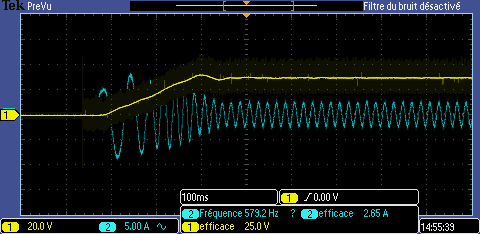
\includegraphics[width=13cm]{titlepage.png}\\
			\vspace{\fill}
			\textbf{Novembre 2021}\\
		\end{center}
	\end{titlepage}
	
	\tableofcontents
	\newpage
	
	\section{Introduction}
	\paragraph{}
	Dans ce tp, nous allons nous intéresser au fonctionnement d’un variateur électronique permettant de faire varier la vitesse d’une machine à courant continu. Le principe de ce variateur est de régler la tension moyenne de l’induit à l’aide d’un pont à thyristors tout en gardant un courant continu fixe et donc un flux constant dans l’inducteur. Nous étudierons chacun des circuits du variateur avant de nous intéresser sur la charge et sur le réseau sur lequel est branché le variateur.
	
	\section{Préparation}
	
		La préparation de ce TP est disponible en annexe.
		
	\section{Manipulation}
	
	\subsection{Analyse du fonctionnement du variateur}
	
	\paragraph{Le pont à diodes pour le circuit d'excitation}
	\paragraph{}
	
	Voici les relevés de Ue et Ie à l’aide de l'oscilloscope : 
	
	\begin{figure}[h]
		\centering
		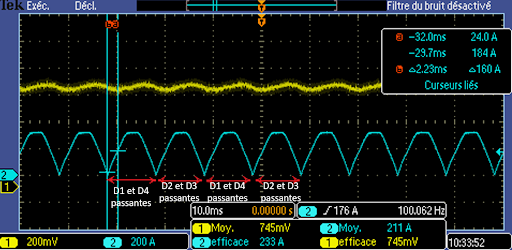
\includegraphics[width=14cm]{pontDeDiodes.PNG}
		\caption{Relevés à la sortie du pont de diodes}
	\end{figure}
	\newpage
	Nous obtenons donc pour les valeurs moyennes 
	$$ U_{e}=211 V, I_{e}=745 mA $$
	Nous obtenons donc d’après la loi d’Ohm : 
	$$ R_{e}=\frac{U_{e}}{I_{e}}=\frac{211}{0.745}=283\Omega $$
	Si l’on observe les deux curseurs verticaux, on voit qu’il y a un très léger déphasage entre le courant et la tension.
	Ce déphasage peut s’expliquer car on a en théorie :  
	$$ U_{e}=R_{e}I_{e}+L_{e}\frac{dI_{e}}{dt} $$
	Or dans notre cas la variation de courant est très faible donc notre circuit est fortement inductif.
	
	\paragraph{Le pont à thyristors pour le circuit d’induit :}
	\paragraph{}
	
	Pour les différentes valeurs de courants et tensions, en toute logique, plus nous augmentons le potentiomètre plus la valeur moyenne du courant et de la tension est importante et plus le bras de la machine tourne vite. 
	Nous avons relevé u(t) et i(t). Nous avons le courant en jaune et la tension en bleu. 
	
	\begin{figure}[h]
		\centering
		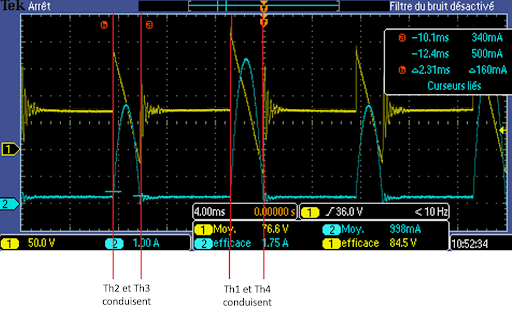
\includegraphics[width=14cm]{pontDeTh.PNG}
		\caption{Relevés à la sortie du pont à Thyristors}
	\end{figure}

	Th1 et Th4 s’amorcent à $\alpha$. Th2 et Th3 s'amorcent à $\alpha+\pi$. 

	Les thyristors sont passants quand la tension est positive à ses bornes et que le courant dans la gâchette est suffisant.
	Les thyristors se bloquent lorsque le courant qui les traverse s’annulent. Les thyristors se bloque donc avec un retard de $\frac{\alpha}{\omega}$. Ce qui explique que la tension est parfois négative sur l'oscilloscope. Pour former une cellule de commutation, la source de tension ne doit pas être en court-circuit et la source de courant en circuit ouvert. Ainsi les Th1 et Th4 s’amorcent en même temps et bloquent Th2 et Th3 et réciproquement.

	A 40\% du potentiomètre, nous avons les valeurs moyennes suivantes:
	$$U= 77.6 V,  I= 865 mA.$$
	
	La fréquence du courant est de 50 Hz, soit une période de 20 ms.
	L’intervalle de conduction d’un transistor est selon la figure précédente de 2.31ms. 
	Nous avons donc un angle de retard de $$\alpha=\frac{2.3}{10}=0.23$$ 
	Soit $$0.23*180 = 41.4°$$
	
	\subsection{Impact du variateur sur l’ensemble moteur-charge}
	\paragraph{Alimentation par le variateur :}
	\paragraph{}
	Nous réglons la charge à sa valeur maximale soit 2,1 kW.
	
	Pour obtenir la caractéristique couple/vitesse du moteur à partir de ces relevés, on peut écrire l’équation suivante: 
	
	$$ e=K\Omega, U=e+RI, C=KI $$
	donc $$ U-RI=K\Omega=\frac{C}{I}\Omega $$
	et donc $$ C=(U-RI)\frac{I}{\Omega} $$

	Ensuite, comme $U=e+RI$ on peut déterminer la valeur de R comme étant $R=\frac{dU}{dI}$.
	Pour cela on peut plot le graph $U=f(I)$ et grâce à une régression linéaire, on obtient approximativement     
	$$U = 516 + 80*I$$on peut alors identifier $R=80$ .
	
	Cela nous permet enfin d'afficher la caractéristique couple/vitesse qui est le suivant:
	\begin{figure}[h]
		\centering
		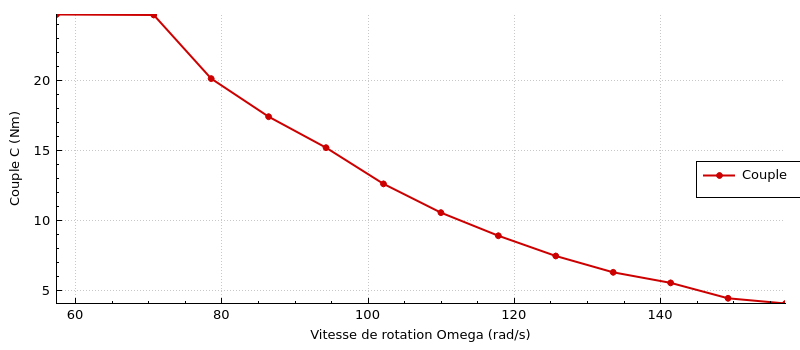
\includegraphics[width=14cm]{plotCdeOmega2.png}
		\caption{Carateristique couple/vitesse}
	\end{figure}

	\paragraph{Type de Charge :}
	\paragraph{}
	
	Le moteur à courant continu doit entraîner la machine synchrone qui peut être représentée par un schéma de type RLE. Cette machine synchrone est elle-même chargée par une charge purement résistive qui ajoute une composante R en série de la charge globale.\\
	Cela nous amène à une charge globale de type RLE avec une composante R forte.
	
	\begin{figure}[h]
		\centering
		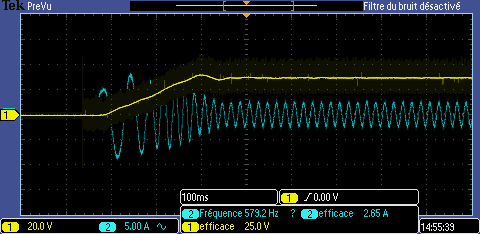
\includegraphics[width=14cm]{titlepage.png}
		\caption{Relevés à la sortie du pont de diodes}
	\end{figure}

	Pour la position 40\% du potentiomètre, nous avons relevé une tension moyenne de 77.1 V, un courant moyen de 4.72A, ce qui permettait à la machine de tourner à environ 550 tr/min. 
	A vide, nous avions presque la même valeur moyenne de tension mais une valeur de courant beaucoup plus faible (environ 5.5 fois inférieur). Cette observation est tout à fait normale et provoquée par la charge puisque pour tourner à la même vitesse le moteur doit consommer plus de courant.

	On peut voir sur l’oscilloscope que le courant varie beaucoup (de 0 à 15-18V environ). Ces fortes ondulations peuvent provoquer un emballement thermique de la machine et donc une usure de celle-ci

	Cependant la vitesse de rotation de la machine n’est pas impactée (constante au cours du temps) car le courant d’induit varie trop rapidement.

	\paragraph{Impact du variateur sur l'alimentation électrique}
	\paragraph{}
	
	\begin{figure}[h]
		\centering
		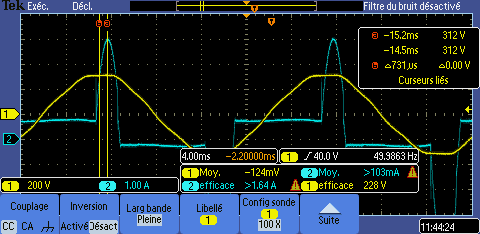
\includegraphics[width=14cm]{TEK00008.PNG}
		\caption{Relevés du réseau}
	\end{figure}

	Nous observons la tension et le courant appelé au réseau, nous n'avons donc ni un courant ni une tension redressés. On observe un léger déphasage entre le courant et la tension.

	Nous mesurons un retard temporel de 731 $\mu s$ ce qui équivaut à un déphasage de 13° entre la tension Ur et le fondamental du courant Ir.

	Nous mesurons :

	$$ V_{eff}=228V, I_{eff}=1.77A $$
	$$ P=1.77*228*cos(13°)=393W $$
	$$ S=V_{eff}*I_{eff}=403VA $$
	
	Le facteur de dimensionnement de notre moteur est donc de 97\%.
	
	D’après la préparation, nous avons $$I_{ra}= I_{eff}*cos(\phi)=1.72 A$$
	La quantité $I_{r1}*cos(\phi)$ correspond à la valeur du courant si il était en phase avec la tension.
	
	\begin{figure}[h]
		\centering
		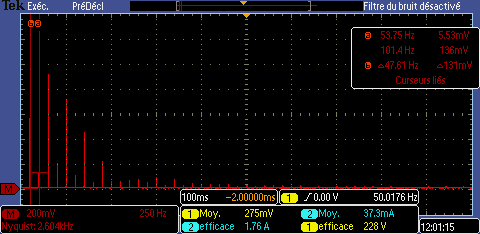
\includegraphics[width=14cm]{TEK00010.PNG}
		\caption{Transformée de fourier du courant réseau}
	\end{figure}

	\begin{center}
	\begin{tabular}{|c|c|}
		\hline
		N° de l'Harminique & Valeur (en mA)\\
		\hline
		1 & 1160\\
		\hline
		2 & 250\\
		\hline
		3 & 950\\
		\hline
		4 & 188\\
		\hline
		5 & 725\\
		\hline
		6 & 100\\
		\hline
		7 & 476\\
		\hline
		8 & 44\\
		\hline
		9 & 228\\
		\hline
		10 & 52\\
		\hline
	\end{tabular}
	\end{center}

	La valeur des harmoniques est bien inférieure à celle imposée par la norme CEI 1000-3-2. Le variateur satisfait la norme mise en vigueur, ce qui est logique étant donné qu’il est commercialisé.
	Les harmoniques se répercutent sur le reste du réseau. S'ils sont trop importants, cela pourrait perturber le réseau et voir endommager d’autres appareils électroniques.\\
	Il a donc été nécessaire d’instaurer une norme concernant les harmoniques de courant. 
	
	\section{Conclusion}
	
	Lors de ce TP, nous avons pu étudier le comportement de l'alimentation par pont de thyristors pour un moteur à courant continu.\\
	Nous avons pu observer le hachage de la tension par le pont de thyristors ainsi que l'influence de la charge sur l'allure de celle-ci avec des déphasages engendrés pas la caracteristique inductive de la charge.\\
	
	Nous avons également pu valider par une étude fréquentielle la conformité de l'alimentation concernant les normes d'utilisation du réseau.\\
	
	\newpage
	\section{Annexes}
	\begin{figure}[h]
		\begin{center}
			\begin{tabular}{|c|c|c|}
				\hline
				I (A) & U(V) & $\Omega$ (tr/min)\\
				\hline
				4.72 & 77.1 & 548\\
				\hline
				5.28 & 92 & 675\\
				\hline
				5.13 & 102 & 750\\
				\hline
				5.08 & 110 & 825\\
				\hline
				5.05 & 120 & 900\\
				\hline
				4.88 & 126 & 975\\
				\hline
				4.75 & 135 & 1050\\
				\hline
				4.63 & 143 & 1125\\
				\hline
				4.51 & 152 & 1200\\
				\hline
				4..4 & 160 & 1275\\
				\hline
				4.36 & 168 & 1350\\
				\hline
				4.2 & 177 & 1425\\
				\hline
				4.23 & 186 & 1500\\
				\hline
			\end{tabular}
		\end{center}
	\caption{Relevés pour le moteur en charge}
	\end{figure}
	
	
	
\end{document}